\chapter{Analysis}

\section{Calibration of the parameters}

Having a lot of parameters to calibrate, we decided to limit the number of possible values for each parameter. This choice was made to reduce the number of simulations to be performed and to have a more manageable number of results to analyze. The parameters that we decided to calibrate are the following:

\begin{itemize}
    \item \texttt{pCpuBound}: \{0.1, 0.9\} \\
          The probability of a process being CPU-bound has two values, one for a system with a high number of I-O bound processes and the other for a system with a high number of CPU-bound processes.
    \item \texttt{meanGenerationTime, meanProcessDuration}:\\
          The mean generation time and process duration were chosen to have a comparable load on the system for both values of \texttt{pCpuBound}. For each value of \texttt{pCpuBound} there is a simulation with heavy load and one with a lighter load. The values are on the order of tenths of a second.
    \item \texttt{numCpus}: \{4, 12\} \\
          The number of CPUs was chosen to simulate quad-core, and newer systems with 12 cores.
    \item \texttt{isFCFS}: \{true, false\} \\
          The scheduling policy that the scheduler uses can be either First-Come-First-Served or Shortest-Job-First.
    \item \texttt{generationType}: \{"exponential", "uniform"\} \\
          In addition to the exponential distribution, we also considered the uniform distribution for the generation of processes.
    \item \texttt{durationType}: \{"exponential", "uniform"\} \\
          In addition to the exponential distribution, we also considered the uniform distribution for the duration of the processes.
\end{itemize}


\section{Time parameters setup}

\subsection{Warm-up period}

To determine the warm-up period, we observed the development of the mean number of busy CPUs over time, through 10 independent runs and with different parameters configurations. The number of busy CPUs is a good indicator of the system's stability, as it doesn't depend on the scheduling policy.
Our observations showed that the system stabilizes well before \SI{200}{\second} in all tested configurations. To handle variability and ensure robustness in worse cases, we set the warm-up period to \SI{200}{\second}.

\begin{figure}[H]
    \captionsetup{type=figure}
    \centering
    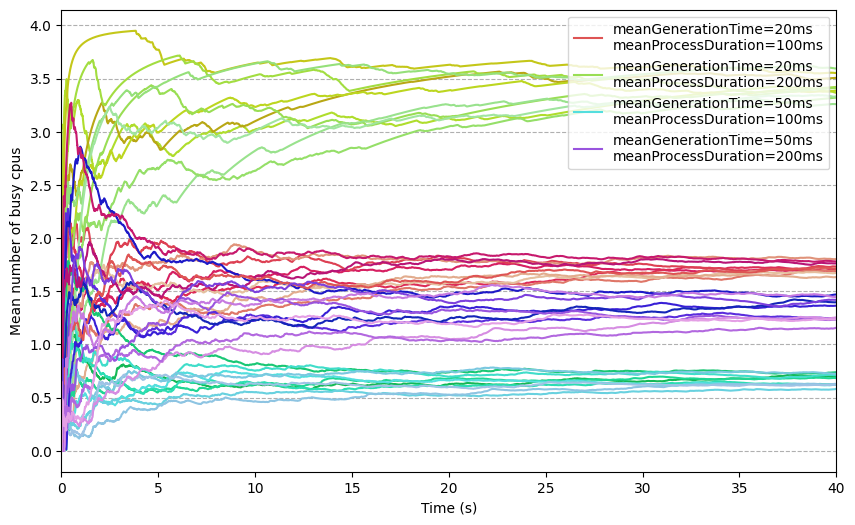
\includegraphics[width=0.9\textwidth]{./images/04/lineWarmup.png}
    \captionof{figure}{Line chart of the mean number of busy CPUs over time for different configurations of meanGenerationTime and meanProcessDuration and multiple repetitions.}
    \label{fig:lineWarmup}
\end{figure}

\begin{figure}[H]
    \captionsetup{type=figure}
    \centering
    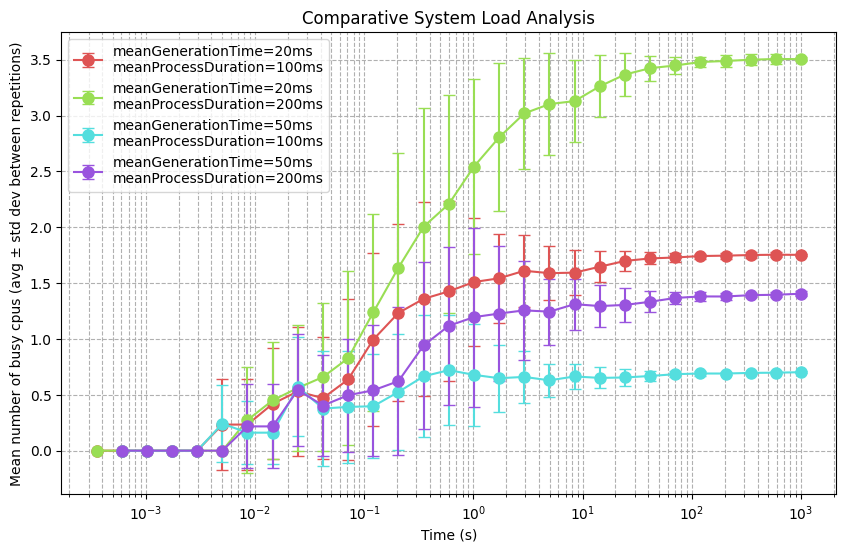
\includegraphics[width=0.9\textwidth]{./images/04/errorWarmup.png}
    \captionof{figure}{Average and Std dev of the mean number of busy CPUs over the repetitions.}
    \label{fig:errorWarmup}
\end{figure}


\begin{table}[H]
    \centering
    \begin{tabular}{c|cc|cc|cc|cc}
                 & \multicolumn{2}{c|}{20ms, 100ms} & \multicolumn{2}{c|}{20ms, 200ms} & \multicolumn{2}{c|}{50ms, 100ms} & \multicolumn{2}{c}{50ms, 200ms}                                   \\
        Time (s) & Avg                              & Std Dev                          & Avg                              & Std Dev                         & Avg  & Std Dev & Avg  & Std Dev \\
        \midrule
        1        & 1.52                             & 0.58                             & 2.54                             & 0.78                            & 0.68 & 0.46    & 1.20 & 0.80    \\
        2        & 1.54                             & 0.37                             & 2.85                             & 0.64                            & 0.67 & 0.27    & 1.25 & 0.51    \\
        5        & 1.59                             & 0.24                             & 3.10                             & 0.46                            & 0.63 & 0.15    & 1.24 & 0.29    \\
        10       & 1.63                             & 0.18                             & 3.18                             & 0.34                            & 0.65 & 0.10    & 1.29 & 0.20    \\
        20       & 1.68                             & 0.11                             & 3.33                             & 0.22                            & 0.64 & 0.08    & 1.27 & 0.15    \\
        50       & 1.72                             & 0.05                             & 3.43                             & 0.10                            & 0.68 & 0.05    & 1.35 & 0.09    \\
        100      & 1.74                             & 0.02                             & 3.47                             & 0.05                            & 0.69 & 0.02    & 1.37 & 0.04    \\
        200      & 1.75                             & 0.02                             & 3.49                             & 0.05                            & 0.69 & 0.02    & 1.38 & 0.03    \\
        500      & 1.75                             & 0.03                             & 3.50                             & 0.05                            & 0.70 & 0.01    & 1.40 & 0.02    \\
        1000     & 1.75                             & 0.01                             & 3.51                             & 0.02                            & 0.70 & 0.01    & 1.41 & 0.02    \\
    \end{tabular}
    \caption{Average and Std dev of the mean number of busy CPUs over the repetitions.}
    \label{tab:stabilization}
\end{table}

\subsection{Simulation duration}

For the simulation duration, we chose to end it at \SI{1000}{\second}. This ensures that after discarding the initial \SI{200}{\second} warm-up period, there remains \SI{800}{\second} of simulation data for analysis. Given that the mean generation time is on the order of tenths of a second, this duration strikes a balance between obtaining statistically meaningful results even after subsampling and maintaining reasonable simulation times.


\section{Subsampling}

To analyze the data, the assumption of IID-ness will be needed, but without further modification the samples do not uphold it.
For instance, if a process finishes with a large turnaround time, which is caused by a long queue, it is likely that the same thing will happen for the next processes.

To address this and ensure independence between samples, subsampling has been employed. The new sample is constructed taking each point of the starting sample with probability $p$.
$p = \frac{1}{2^k}$ and $k$ is the smallest integer that passes the Ljung-Box test.
Using the Ljung-Box test makes it possible to automate the subsampling step. It was implmented to test the first 30 lags, with a significance level of 5\%, with these values the sample is considered independent if:
\vspace{-0.5\baselineskip}
\begin{equation}
    Q = n(n+2) \sum_{k=1}^{30} \frac{\hat{\rho}_k^2}{n-k} < \chi^2_{0.95,30} \approx 43.77
\end{equation}
The closer the system is to saturation, the stronger the correlation becomes as it can be seen in \cref{fig:autoCorComparison}.

% todo dare nomi ai grafici con metrica che ti dice quanto saturo (bello se definita nella parte iniziale)
\begin{figure}[H]
    \captionsetup{type=figure}
    \centering
    \begin{subfigure}[b]{0.45\textwidth}
        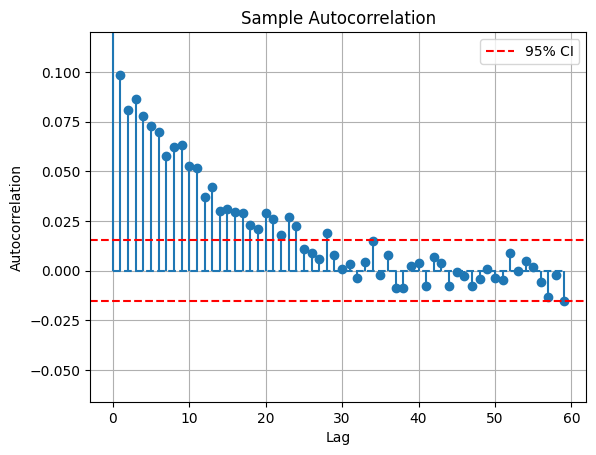
\includegraphics[width=\textwidth]{./images/04/autoCorHighUnfix.png}
        \caption{System close to saturation. Q = 1099}
        \label{fig:autoCorHighUnfix}
    \end{subfigure}
    \hfill % Add space between the subfigures
    \begin{subfigure}[b]{0.45\textwidth}
        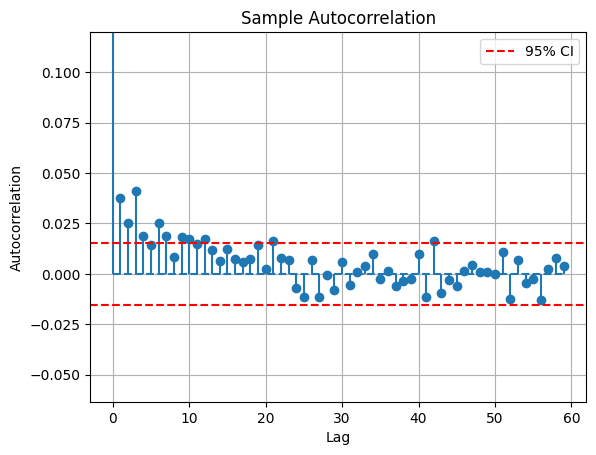
\includegraphics[width=\textwidth]{./images/04/autoCorLowUnfix.png}
        \caption{System with high load. Q = 129}
        \label{fig:autoCorLowUnfix}
    \end{subfigure}
    
    \vspace{10pt} % Add vertical space between the two rows
    
    \begin{subfigure}[b]{0.45\textwidth}
        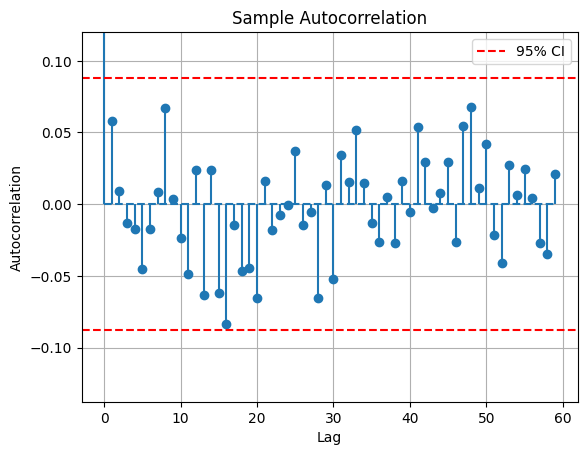
\includegraphics[width=\textwidth]{./images/04/autoCorHighFix.png}
        \caption{System close to saturation with $p=1/16$. Q = 25}
        \label{fig:autoCorHighFix}
    \end{subfigure}
    \hfill % Add space between the subfigures
    \begin{subfigure}[b]{0.45\textwidth}
        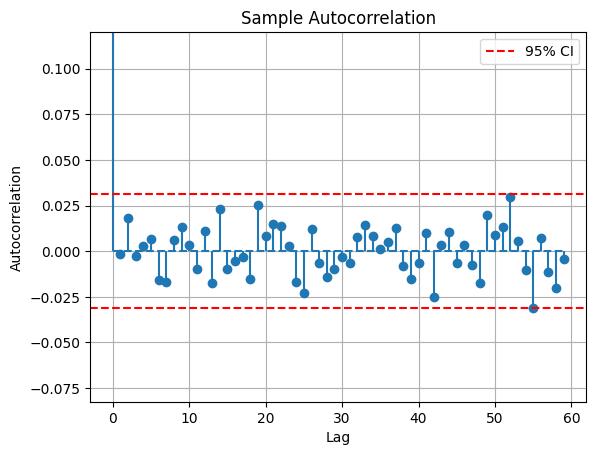
\includegraphics[width=\textwidth]{./images/04/autoCorLowFix.png}
        \caption{System with high load with $p=1/4$. Q = 20}
        \label{fig:autoCorLowFix}
    \end{subfigure}
    
    \vspace{10pt} % Add vertical space before the caption
    \caption{Comparison of turnaround time autocorrelation with and without subsampling for different loads.}
    \label{fig:autoCorComparison}
\end{figure}

\section{Statistical analysis}

For each of our measurements we made sure that the sample variance was stable for different simulation time, proving that the variance of the measurements is finite, and for each of them we collected more than 500 samples. Since after subsampling our observations are IID we can use the central limit theorem to state that:

% todo cambiare e usare direttamente la formula del CI

\begin{equation}
    Z = \frac{\overline{X} - \mu}{\frac{S}{\sqrt{n}}} \sim N(0,1)
\end{equation}

We chose to use a confidence interval of 95\% for our analysis.

\subsection{First-Come-First-Served}
\subsubsection{Turnaround time}

\begin{figure}[H]
    \captionsetup{type=figure}
    \centering
    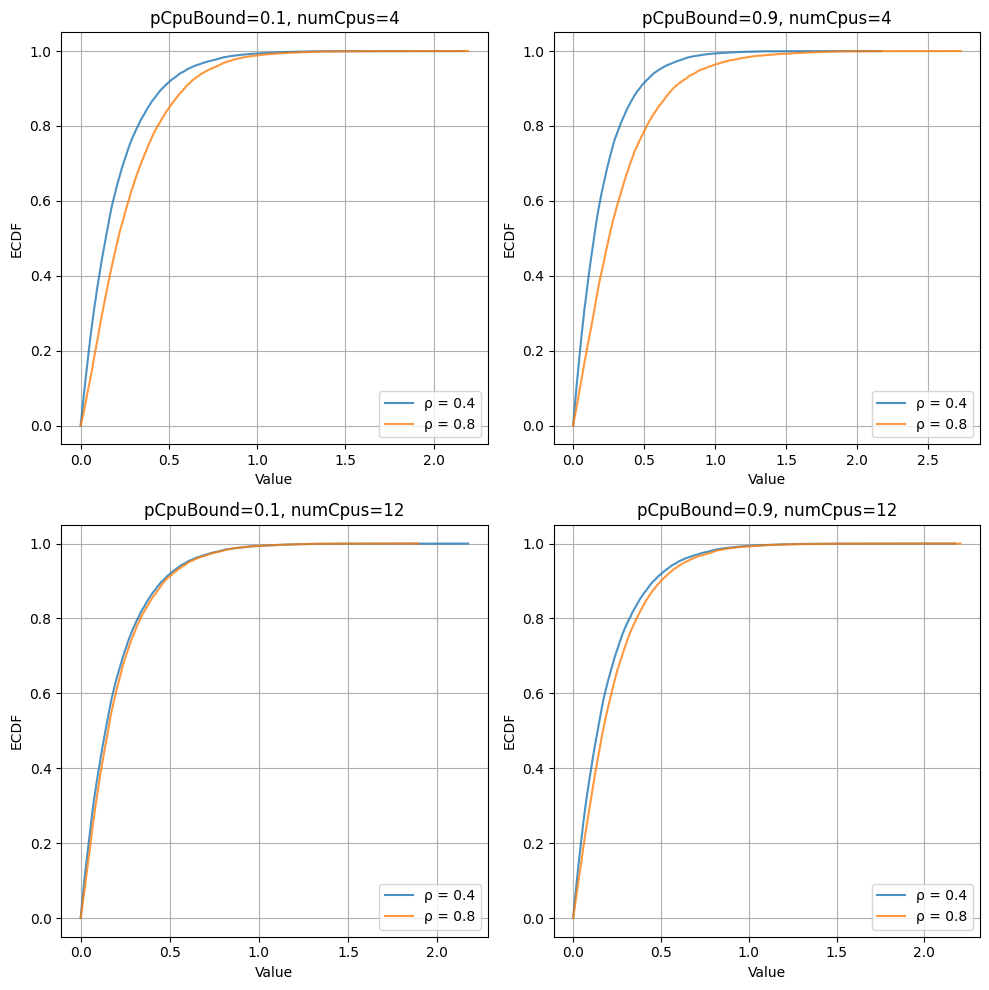
\includegraphics[width=0.9\textwidth]{./images/04/fcfs/ecdf.png}
    \caption{Empirical CDF of the turnaround time for different configurations of the system.}
    \label{fig:fcfs_ecdf}
\end{figure}

\begin{figure}[H]
    \captionsetup{type=figure}
    \centering
    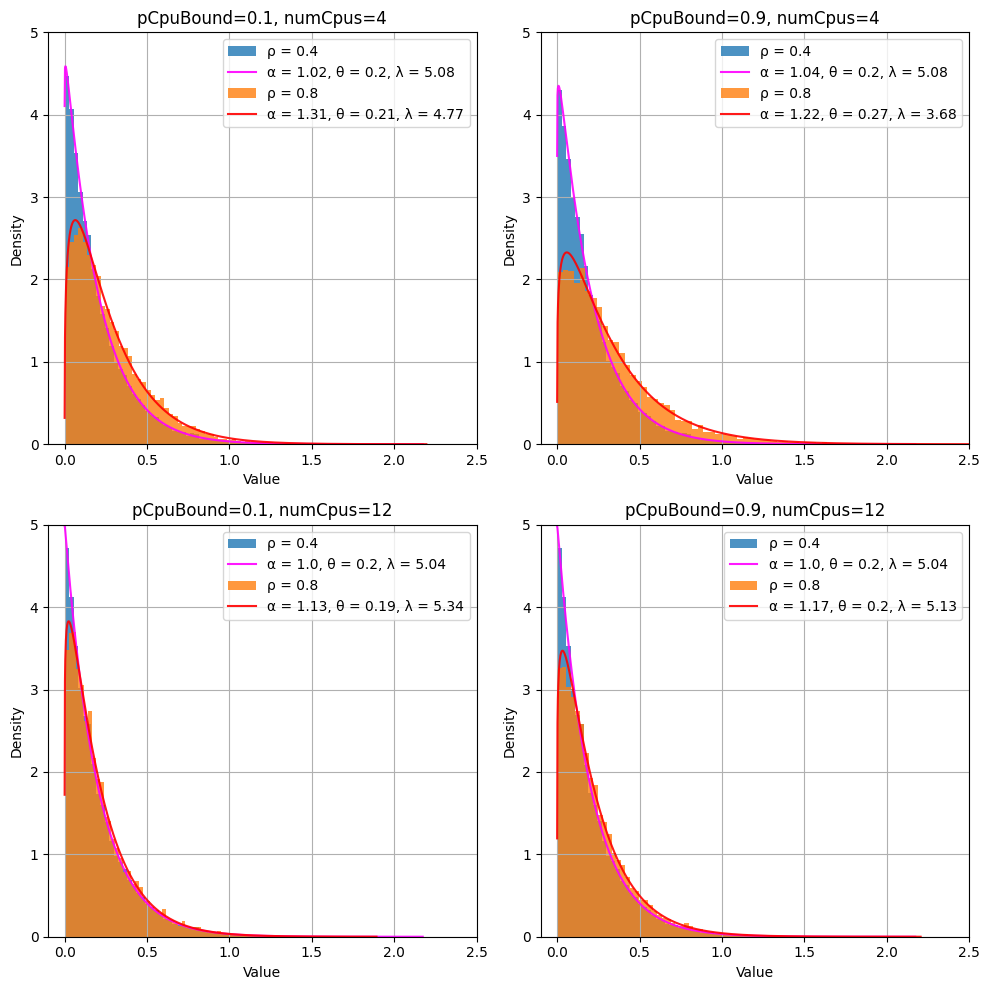
\includegraphics[width=0.9\textwidth]{./images/04/fcfs/density.png}
    \caption{Density plot of the turnaround time for different configurations of the system.}
    \label{fig:fcfs_density}
\end{figure}

\begin{figure}[H]
    \captionsetup{type=figure}
    \centering
    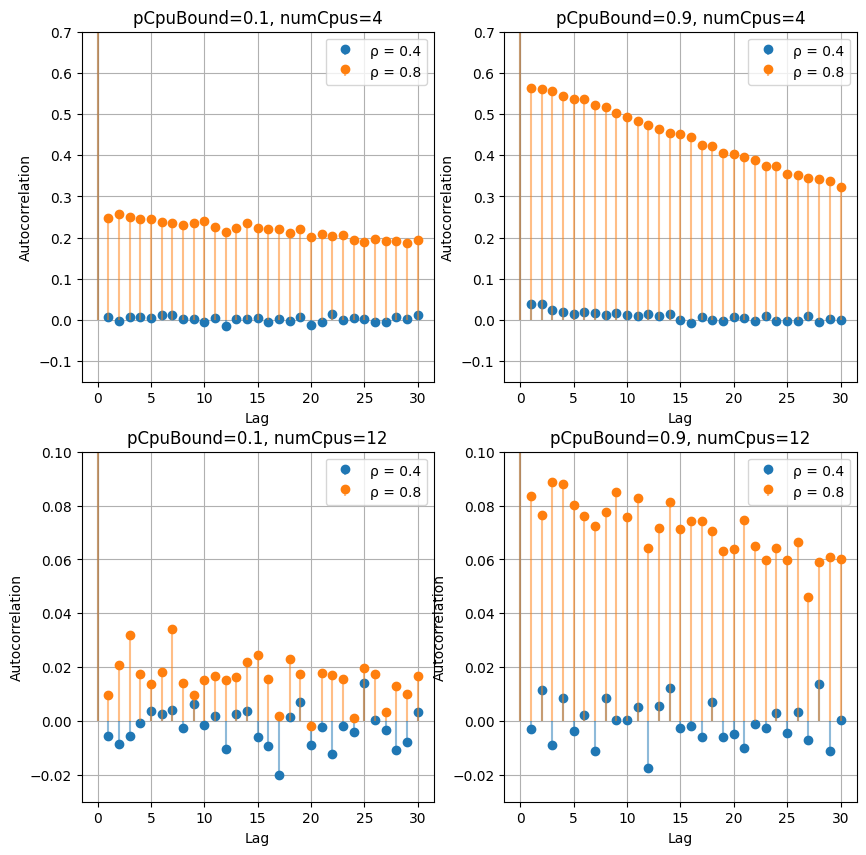
\includegraphics[width=0.9\textwidth]{./images/04/fcfs/autocorrelation.png}
    \caption{Autocorrelation plot of the turnaround time for different configurations of the system.}
    \label{fig:fcfs_autocorrelation}
\end{figure}

\begin{figure}[H]
    \captionsetup{type=figure}
    \centering
    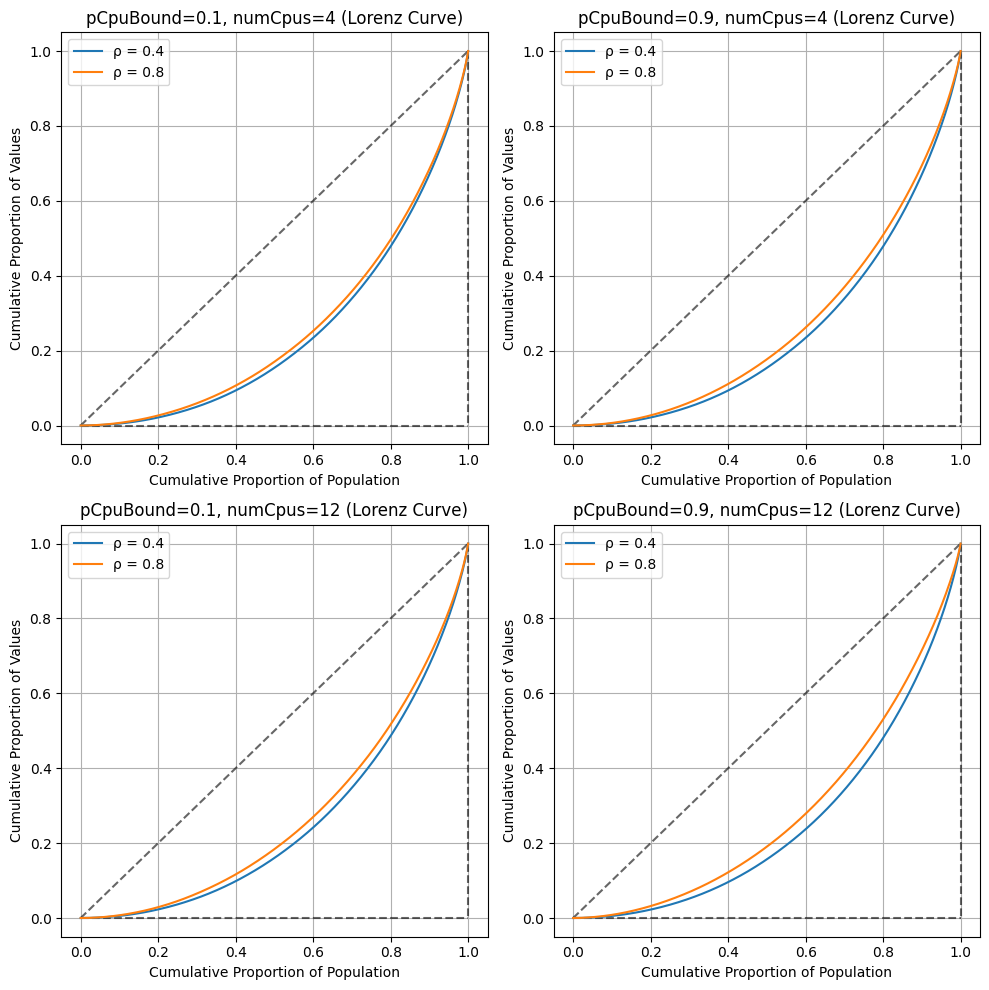
\includegraphics[width=0.9\textwidth]{./images/04/fcfs/lorenz.png}
    \caption{Lorenz curve of the turnaround time for different configurations of the system.}
    \label{fig:fcfs_lorenz}
\end{figure}

\subsubsection{Response time}
\subsubsection{Throughput}
\subsubsection{CPU utilization}
\subsection{Shortest-Job-First}